% --
% my cv

\documentclass[11pt, a4paper]{article}

% add packages and macros
% --
% packages

% language packages
\usepackage[german, english]{babel}

\usepackage[utf8]{inputenc}
%\usepackage{parallel, enumitem}

% tabular settings
\usepackage{tabularx}

% figures
\usepackage{graphicx}

% html color
\usepackage[dvipsnames]{xcolor}

% hyperreferences
\usepackage[colorlinks=true, urlcolor=viola]{hyperref}

% skip intend
\usepackage{parskip}

% two collumns
\usepackage{multicol}

% graphics
%\usepackage{flafter}
%\usepackage{placeins}
%\usepackage{float}
%\usepackage{psfrag}
%\usepackage{wrapfig}

% fonts
\usepackage[light, math]{kurier}
\usepackage[T1]{fontenc}

% geometry
\usepackage{geometry}

% enquotes
\usepackage{csquotes}

\usepackage{array}

% language if package
\usepackage{iflang}

% enumeration stuff
\usepackage{enumitem}
\setlist[enumerate]{label=(\roman*), topsep=0pt, itemsep=0pt, parsep=0pt, nosep}
% --
% macros

% macros
\newcommand{\headParam}[1]{{\hspace{-0.10cm}\fontfamily{ffm}\selectfont \textbf{\Large{#1}}}}
\newcommand{\fancyName}[1]{{\normalfont \selectfont \textbf{\Huge{#1}}}}
\newcommand{\myTitle}[1]{{\fontfamily{ffm}\selectfont \textbf{\Huge{#1}} }}
\newcommand{\mySubTitle}[1]{{\fontfamily{ffm}\selectfont \textbf{\large{#1}} }}

% colors
\definecolor{tronBlue}{HTML}{6FC3DF}
\definecolor{tronOrange}{HTML}{DF740C}
\definecolor{grela}{RGB}{109, 199, 177}
\definecolor{yeola}{RGB}{217, 175, 107}
\definecolor{viola}{RGB}{185, 83,  126}

% placement in tables
\newcolumntype{M}[1]{>{\centering\arraybackslash}m{#1}}

% two columns
\setlength{\columnsep}{1cm}

%\newcommand*{\myfont}{\fontfamily{<familyname>}\selectfont}

% set paper geometry: A4 210 x 297
\geometry{a4paper, total={160mm, 257mm}, left=25mm, top=20mm}

% empty page style
\pagestyle{empty}

% complex image tool
\usepackage{tikz}


% --
% document

\begin{document}
%\selectlanguage{german}
\selectlanguage{english}
% --
% overlay image
\begin{tikzpicture}[remember picture, overlay, opacity=1.0]
  \node at (current page.north) [yshift=-13mm] {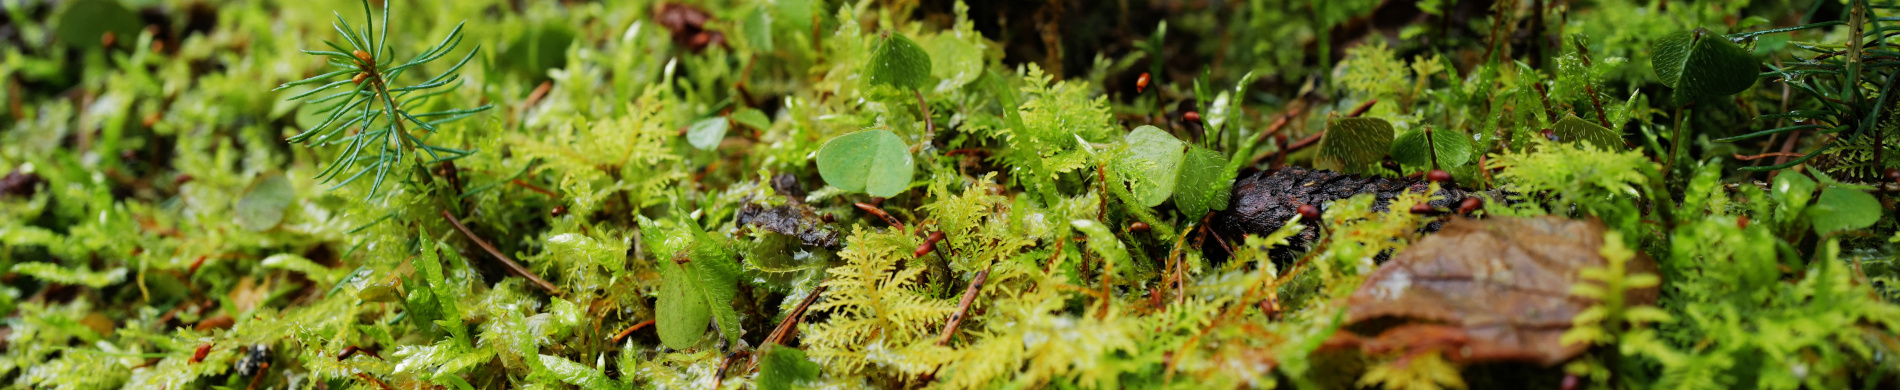
\includegraphics[width=1.4\textwidth]{./figs/green.jpg}};
\end{tikzpicture}
% --
% header
\vspace{-0.5cm}
\begin{multicols}{2}

  % my image
  \begingroup \centering 
\includegraphics[width=0.4\textwidth]{./figs/chris_transparent.png} \endgroup\\

  \vspace{0.9cm}
  % fancy name
  \fancyName{Christian Walter}\\\\
  \headParam{\IfLanguageName{german}{Kontakt}{Contact}}\\\\
  % contact
  \begin{tabular} { l l }
    \textbf{E-Mail:} & \href{mailto:christian.walter@mailfence.com}{christian.walter@mailfence.com}\\
    \textbf{\IfLanguageName{german}{Telefon:}{Phone:}} & +43 680 210 423 1\\
    \textbf{\IfLanguageName{german}{Adresse:}{Address:}} & Neuhof 13, 3631 Ottenschlag\\
  \end{tabular}
\end{multicols}
% --
% content
\begin{multicols}{2}
  % inputs
  % --
% personal

\IfLanguageName{german}
{

\headParam{Information zur Person}

\begin{tabular} { l p{3.9cm} }
  \textbf{Geschlecht:} & Männlich\\
  \textbf{Nationalität:} & Österreich\\
  \textbf{Geburtsjahr:} & 1991\\
  \textbf{Geburtsort:} & Zwettl\\
\end{tabular}

\textbf{Ein paar Worte über mich:}\\
Ich bin ein freundlicher und aufgeschlossener Mensch und verbringe gerne meine Freizeit mit Freunden bei einem guten Kaffee.\\

% --
% languages

\headParam{Fremdsprachen}\\\\
\begingroup \centering \includegraphics[width=0.25\textwidth]{./figs/languages.jpg} \endgroup\\


% --
% skills

\headParam{Freizeitbeschäftigungen}\\
Brett- und Videospiele, Brot backen, Reisen, Fotografie, Laufen, Slacklinen, Klettern, Mountainbiken, Lesen, Piano, Gitarre, \dots\\

% --
% technical skills

\headParam{Technische Fertigkeiten}\\
Programmieren (Python, C, C++), Maschinelles Lernen, Spiele Entwicklung, Audio Verarbeitung, Automatische Spracherkennung, Maschinelles Sehen, 3D-Modellierung, Elektronik, \dots\\

% --
% software skills

\headParam{Software Fertigkeiten}\\
Blender, Unity3D, \LaTeX, Inkscape, Gimp, \dots
}
{
% --
% personal information

\headParam{Personal Information}

\begin{tabular} { l p{3.9cm} }
  \textbf{Gender:} & Male\\
  \textbf{Nationality:} & Austria\\
  \textbf{Year of birth:} & 1991\\
  \textbf{Place of birth:} & Zwettl\\
\end{tabular}

\textbf{Few words about myself:}\\
I'm a friendly and open minded person who enjoys to share his free time with friends, preferably at a cup of hot coffee and a board game at hand.
I also like being in nature and travel to incredible places, where I capture these moments with my leica camera or record audio of nature sounds. 
I love game development (usually at game jams) and nowadays I look much into bioacoustics.\\

% --
% languages

\headParam{Foreign Languages}\\\\
\begingroup \centering \includegraphics[width=0.25\textwidth]{./figs/languages.jpg} \endgroup\\
%\begingroup \centering \includegraphics[width=0.4\textwidth]{./figs/tron_blue01_cut.png} \endgroup


% --
% skills

\headParam{Hobbies}\\
Board and video games, bread baking, travelling, photography, running, slacklining, climbing, mountain bike, reading, piano, guitar, \dots\\

% --
% technical skills

\headParam{Technical Skills}\\
Programming (Python, C, C++), machine learning, game development, audio processing, automatic speech recognition, computer-vision, 3D modelling, electronics, \dots\\

% --
% software skills

\headParam{Software Skills}\\
Blender, Unity3D, \LaTeX, Inkscape, Gimp, \dots
}
  \columnbreak
  % --
% education

\headParam{Education}

% vs ottenschlag
\textbf{Volksschule Ottenschlag}\\
\texttt{(09/1997 - 06/2001)}

% hs ottenschlag
\textbf{Hauptschule Ottenschlag}\\
\texttt{(09/2001 - 06/2005)}

% htl st. pölten
\textbf{HTL St. Pölten}\\
\texttt{(09/2005 - 06/2010)}\\
Electrical Engineering

% university
\textbf{Technical University Graz}\\
\texttt{(10/2014 - 03/2022)}\\
BSc Electrical Engineering\\
BSc Electrical Engineering and Audio Engineering\\
MSc Individual Master's program: Information and Computer Engineering

% exchange
\textbf{University of Oulu (Finland)}\\
\texttt{(08/2016 - 03/2017)}\\
Exchange semester\\
  % --
% working experience

\IfLanguageName{ngerman}
{

% title
\headParam{Arbeitserfahrung}

\textbf{Alpin Innovation+Technik / Alpin Umwelttechnik}\\
\texttt{(08/2010 - 11/2021)}\\
Steuerungstechniker (Voll- und Teilzeit)

\textbf{Trumpf Maschinen Austria}\\
\texttt{(06/2012 - 09/2014)}\\
Steuerungstechniker (Vollzeit)

\textbf{Institute of Advanced Research in Artificial Intelligence (IARAI)}\\
\texttt{(02/2022 - 08/2022)}\\
Praktikum in der Verkehrsvorhersage (geringfügig)
}
{

% title
\headParam{Working Experience}

\textbf{Alpin Innovation+Technik / Alpin Umwelttechnik}\\
\texttt{(08/2010 - 11/2021)}\\
Electrical control engineer (full and part time)

\textbf{Trumpf Maschinen Austria}\\
\texttt{(06/2012 - 09/2014)}\\
Electrical control engineer (full time)

\textbf{Institute of Advanced Research in Artificial Intelligence (IARAI)}\\
\texttt{(02/2022 - 08/2022)}\\
Internship in traffic forecast (marginal employment)
}
  % game dev (optional)
  %\input{./game_dev.tex}
\end{multicols}
\newpage
\vspace*{0.75cm}
\headParam{Chronologic Events and Details}\\\\
\begin{tabularx}{\columnwidth}{>{\centering\arraybackslash}p{1.5cm} | p{12cm}}
  \texttt{09/1997} & Volksschule Ottenschlag until \texttt{06/2001}.\\
  \texttt{09/2001} & Hauptschule Ottenschlag until \texttt{06/2005}.\\
  \texttt{09/2005} & HTL St. Pölten: Electrical Engineering with \enquote{Matura} graduation on \texttt{06/2010}.\\
  \texttt{08/2006} & Herbert Wania Elektroinstallationsges.m.b.H: Holiday internship in electrical installation for 1 month.\\
  \texttt{08/2008} & Volk Ges.m.b.H: Holiday internship in electrical installation for 1 month.\\
  \texttt{07/2010} & Alpin Innovation+Technik GmbH: Electrical engineer for wastewater treatment plants (full time) until \texttt{10/2010}.\\
  \texttt{10/2010} & Military service (paramedic) in Zwölfaxing and St. Pölten until \texttt{04/2011}.\\
  \texttt{04/2011} & Alpin Innovation+Technik GmbH: Electrical control engineer for wastewater treatment plants (full time) until \texttt{12/2011}.\\
  \texttt{11/2011} & Volunteering as paramedic at \enquote{Rotes Kreuz} (2 services a month) until \texttt{10/2014}.\\
  \texttt{01/2012} & Alpin Umwelttechnik: Software maintenance and support (marginal employment) until \texttt{10/2014}.\\
  \texttt{06/2012} & Trumpf Maschinen Austria: Electrical control engineer in series production of metal bending machines (full time) until \texttt{09/2014}.\\
  \texttt{10/2014} & Alpin Umwelttechnik: Software maintenance and support (part time) until \texttt{11/2021}.\\
  \texttt{10/2014} & TuGraz: Begin of Bachelor's program Electrical Engineering.\\
  \texttt{10/2015} & TuGraz: Begin of Bachelor's program Electrical Engineering and Audio Engineering.\\
  \texttt{08/2016} & University of Oulu: Exchange semester in Finland until \texttt{03/2017}.\\
  \texttt{12/2018} & TuGraz: Graduation of Bachelor's program Electrical Engineering. Earned academic degree: \enquote{BSc}.\\
  \texttt{12/2018} & TuGraz: Begin of Individual Master's program \enquote{Immersive Human-Technology} in Information and Computer Engineering.\\
  \texttt{11/2020} & TuGraz: Graduation of Bachelor's program Electrical Engineering and Audio Engineering. Earned academic degree: \enquote{BSc}.\\
  \texttt{02/2022} & IARAI: Internship in traffic forecast to evaluate competition models (10h / week) until \texttt{08/2022}.\\
  \texttt{03/2022} & TuGraz: Graduation of Individual Master's program \enquote{Immersive Human-Technology}. Earned academic degree: \enquote{Dipl.-Ing} which is equivalent to \enquote{MSc.}.\\
  \texttt{06/2022} & Traveling around the world until \texttt{04/2023}.\\
\end{tabularx}
\end{document}